%       $Id: grafiken.tex,v 1.11 2004/08/02 11:33:02 bronger Exp $    
%
%     grafiken.tex -- Part of the LaTeX Tutorium
%     Copyright 2004 Project Members of
%                    http://sourceforge.net/projects/latex-tutorium/
%                    
%
%   This program is free software; you can redistribute it and/or
%   modify it under the terms of the Artistic License 2.0 as published
%   by Larry Wall.  You should have received a copy of the Artistic
%   License 2.0 along with this program in the file COPYING; if not,
%   you can get it at
%     http://dev.perl.org/rfc/346.html
%   or contact the current maintainers of the LaTeX Tutorium.
%
%   This program is distributed in the hope that it will be useful, but
%   WITHOUT ANY WARRANTY; without even the implied warranty of
%   MERCHANTABILITY or FITNESS FOR A PARTICULAR PURPOSE.  See the
%   Artistic License 2.0 for more details.
%
%   This file may only be distributed together with a copy of the LaTeX
%   Turorium.
%
%   The LaTeX Tutorium consists of all files listed in manifest.txt.


\section{Grafiken}
\label{sec:Grafiken}

Grafiken werden mit dem Men�-Punkt "`Einf�gen--Grafik"' eingef�gt oder mit
\Alt+\Ctrl+\keystroke A (f�r "`Abbildung"').  Es �ffnet sich dann das
Dialogfenster von Abbildung~\vref{fig:Grafiken}.

\begin{figure}
  \centering
  
\includegraphics{abbildungen}
  \caption{Das Dialogfenster zum Einf�gen von Grafiken}
  \label{fig:Grafiken}
\end{figure}

Man gibt dort zuerst den Dateinamen der Bilddatei an.  Daf�r muss man die
Grafik aus dem Programm, mit dem man die Grafik erstellt hat (z.\,B. Corel
Draw, Photopaint, Excel oder die DigiCam-Software) erst einmal
\emph{exportieren}, damit man eine Datei erh�lt.  Das h�ngt stark vom Programm
ab, meist geht es �ber das Men� "`Datei--Exportieren"'.  Dann kann man f�r
gew�hnlich die Art der Grafikdatei w�hlen.


\subsection*{Einschub: Grunds�tzliches zu Bilddateien}

Es gibt viele Arten von Bilddateien; \LaTeX{} kann \JPEG"~, \PDF- und
\PNG-Dateien direkt in einen Text einbetten:
\begin{description}
\item[\JPEG] ist f�r Fotos und �hnliches gedacht.  Die Dateien
  haben meistens die Endung ``\verb|.jpg|''.
\item[\PDF] ist eigentlich ein Dateiformat f�r ganze Dokumente.  \LaTeX{}
  erzeugt am Ende ja selber ein \PDF\@.  Man kann aber auch einzelne Grafiken
  als \PDF{} abspeichern, z.\,B. mit Corel Draw oder Excel.  Wie das geht,
  steht in Anhang~\vref{sec:FreePDF-usage}\@.  Dieses Format sollte man f�r
  Diagramme oder schematische Zeichnungen benutzen.
\item[\PNG] schlie�lich ist auch f�r Zeichnungen geeignet, hat aber eine
  geringere Qualit�t als \PDF\@.  Es ist daher eher eine Notl�sung, oder f�r
  spezielle Zwecke.
\end{description}
Es gibt noch viele andere Arten von Bilddateien.  Sie m�ssen, damit sie mit
\LaTeX{} verwendbar sind, als \PDF{} abgespeichert werden (siehe wiederum
Anhang~\ref{sec:FreePDF-usage})\@.

\nopagebreak
\noindent\hbox to \linewidth{\large\itshape\hfill Einschub Ende}
\bigskip

\begin{figure}
  \centering
  
\includegraphics{loewe}
  \caption{Ein L�we, \LaTeX{}s Wappentier}
  \label{fig:L�we}
\end{figure}

\noindent
Wenn man die Bilddatei angegeben hat, kann man noch eine Bildunterschrift und
eventuell eine Marke eingeben (f�r Querverweise, siehe
Seite~\pageref{sec:Querverweise}), und dann auf "`OK"' dr�cken.  Der Editor
f�gt dann die notwendigen Befehle in den Text ein:
\begin{lstlisting}
\begin{figure}
  \centering
  
\includegraphics{loewe.jpg}
  \caption{Ein L�we, \LaTeX{}s Wappentier}
  \label{fig:L�we}
\end{figure}
\end{lstlisting}
Das Ergebnis sieht man in Abbildung~\vref{fig:L�we}.


\subsection{Gleitende und nicht-gleitende Abbildungen}
\label{sec:Gleitobjekte}

Was wir gerade eingef�gt haben, war eine sogenannte \emph{gleitende Abbildung}.
Das ist eine Abbildung, f�r die \LaTeX{} den passenden Ort selber sucht.  Man
kann dieses Verhalten auch beeinflussen, daf�r sind die Felder unter
"`Position"' in der Dialogbox da.  Alles, was man dort markiert, sind erlaubte
Positionen f�r die Abbildung.

\begin{wrapfigure}{r}{5cm}
  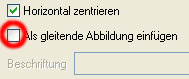
\includegraphics{tabelle1}
\end{wrapfigure}
Eine gleitende Abbildung ist zwar etwas ungemein praktisches, und in den
meisten F�llen nutzt man das auch.  Aber manchmal will man einfach nur eine
Grafik an der aktuellen Position im Text haben.  Dann muss man die Option "`Als
gleitende Abbildung einf�gen"' abw�hlen.  Allerdings ist es dann nicht mehr
m�glich, eine Bildunterschrift zu setzen.


%%% Local Variables: 
%%% mode: latex
%%% TeX-master: "latex-tutorium"
%%% End: 
